\documentclass{beamer}
\usepackage{preamble_beamer}


\title[Функция полезности]{Лекция 2. Теория принятия решений или модель рынка одного агента} % The short title appears at the bottom of every slide, the full title is only on the title page


\begin{document}

\begin{frame}
\titlepage 
\end{frame}

\begin{frame}
\frametitle{Карта курса} 

\begin{itemize} 
    \item \textbf{Введение в финансовый мир} - зачем нужны финансы? 
    \item \textbf{Экономика} - как моделируются агенты и рынки?
    \item \textbf{Финансы} - как определяется стоимость финансовых инструментов? 
    \item \textbf{Деривативы} - модели определения стоимости разных финансовых инструментов

\end{itemize}
\end{frame}

\begin{frame}
  \centering
\Large Примеры
\end{frame}

\begin{frame}{Пример 1: выигрыш случайного контракта}
    
\end{frame}


\begin{frame}{Пример 2: подготовка к экзамену}
\begin{table}
    \centering
    \begin{tabular}{cc}
        Время подготовки & полезность\\
        1 & 100\\
        2 & 200\\
        3 & 300 \\
        100 & 100$\cdot$ 100? \\
    \end{tabular}
    \label{tab:my_label}
\end{table}
\end{frame}

\begin{frame}{Пример 3: баня}

\end{frame}

\begin{frame}
  \centering
\Large Отношение предпочтения
\end{frame}

\begin{frame}{Маршрут лекции}
    \begin{table}[]
\begin{tabular}{l|l|l}
Аксиома & Контрпример & Модель предпочтений                \\ \hline
Полнота      & Частичный порядок & Полное бинарное отношение     \\
Транзитивность   & Парадокс Кондорсе & Диск. функция полезности на дискретном пространстве                   \\
Непрерывность & Лексикограф. порядок & Функция полезности               \\
Независимость  & Парадокс Алле & Ожидаемая функция полезности
\end{tabular}
\end{table}
\end{frame}

\section{Рынок с одним агентом: функция полезности}

\begin{frame}{Рынок с одним агентом: функция полезности}
  \centering
\Large Как моделировать предпочтения (выбор между альтернативами)? 
\end{frame}


\begin{frame}{Векторное представление потребительской корзины}

\begin{columns}
    \column{0.5\linewidth}
    \begin{itemize}
        \item $a=(a_0,\ldots, a_n)\in A$ - набор товаров/портфель
        \item $A$ - множество портфелей
    \end{itemize}


\column{0.5\linewidth}
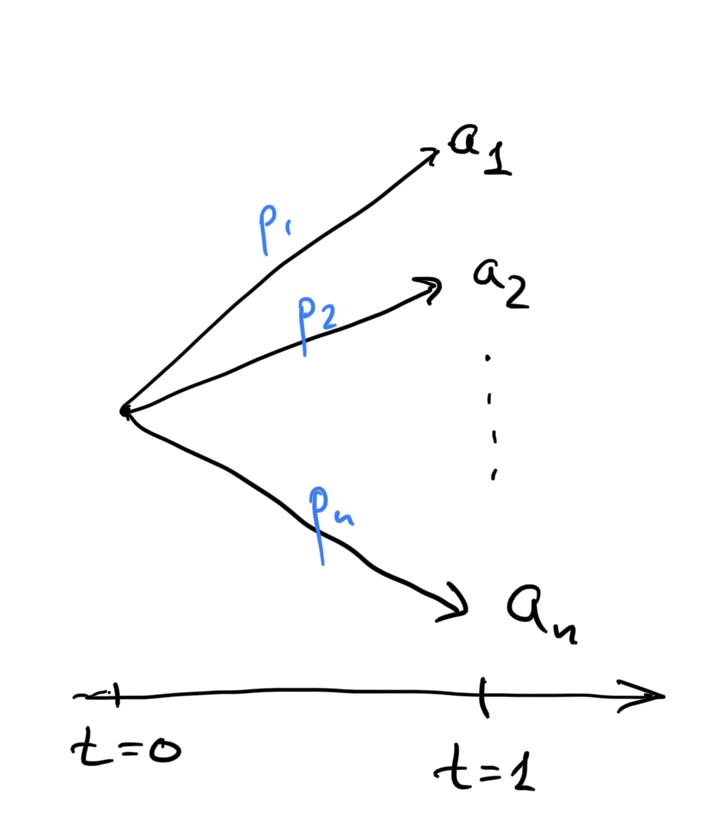
\includegraphics[width=0.5\textwidth]{2_figs/oneperiod.jpeg}
\end{columns}

\end{frame}

\begin{frame}{Векторное представление финансовых инструментов}

\begin{columns}
    \column{0.5\linewidth}
    \begin{itemize}
        \item $a=(a_0,\ldots, a_n)\in A$ - выплаты в разных состояниях мира (payoff)
        \item $A$ - множество допустимых инструментов
    \end{itemize}


\column{0.5\linewidth}
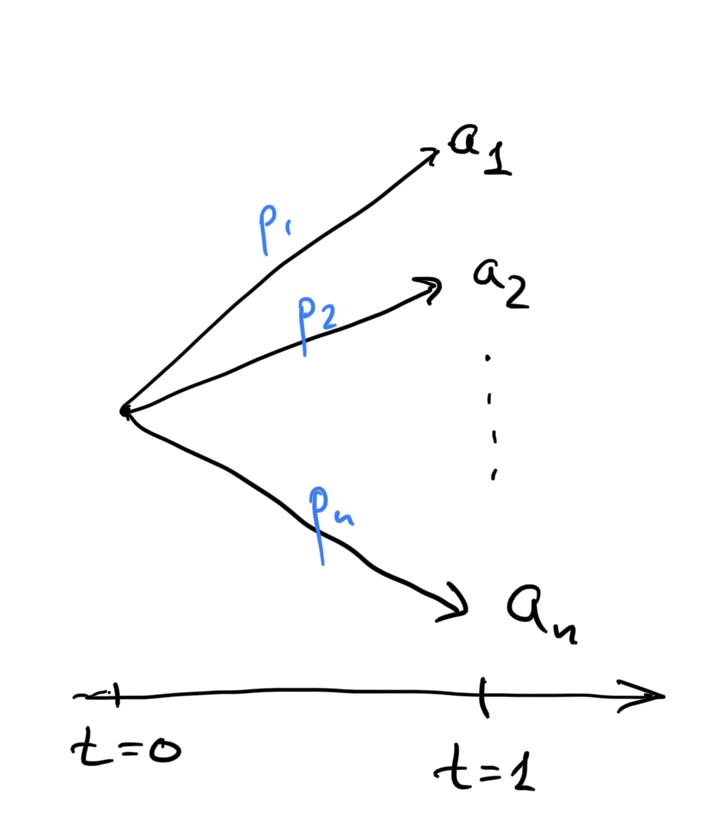
\includegraphics[width=0.5\textwidth]{2_figs/oneperiod.jpeg}
\end{columns}

Финансовый инструмент в однопериодной модели/Лотерея $\sim$ Случайная величина

Финансовый инструмент в многопериодной модели $\sim$ Случайный вектор/последовательность

Финансовый инструмент в непрерывной модели $\sim$ Стохастический процесс

\end{frame}


\begin{frame}{Отношение предпочтения}

\begin{columns}
    \column{0.5\linewidth}
    \begin{itemize}
        \item $a=(a_0,\ldots, a_n)\in A$ - альтернатива
        \item $A$ - множество допустимых альтернатив (портфелей)
        \item $a \preceq b$ - отношение предпочтения
    \end{itemize}


\column{0.5\linewidth}
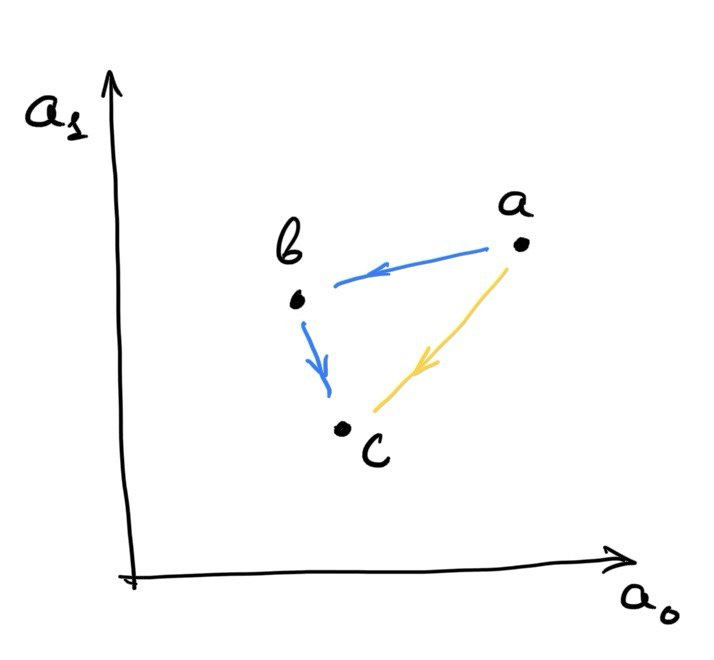
\includegraphics[width=0.75\textwidth]{2_figs/transitivity.jpg}
\end{columns}


\begin{block}{Определение}
Отношение предпочтения рационально, если задается бинарным отношением предпорядка:
    \begin{itemize}
    \item Полнота: $\forall a, b: a \preceq b \lor b \preceq a$ 
    \item Транзитивность: $ a \preceq b \land b \preceq c \Rightarrow  a \preceq c$
\end{itemize}
\end{block}

    
\end{frame}


\begin{frame}{Функция полезности}

\begin{columns}
    \column{0.5\linewidth}
    \begin{block}{Определение}
Пусть $A$ - множество предпочтений. Отношение задается 
$u: A \to \R$ - функцией полезности, если
$$
a \preceq b \Leftrightarrow u(a) \geq u(b)
$$
\end{block}

\column{0.4\linewidth}
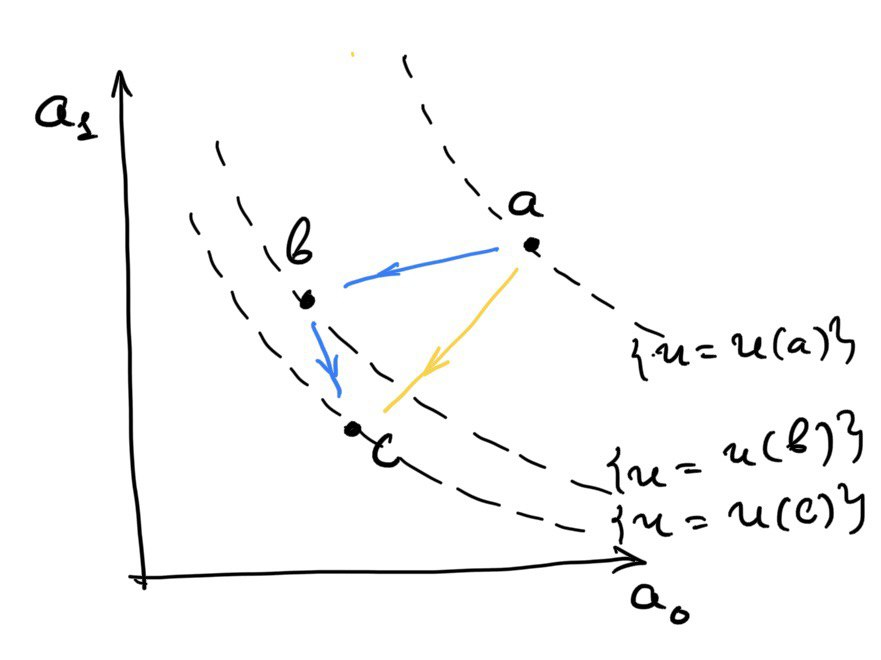
\includegraphics[width=1\textwidth]{2_figs/utility_ordering.jpg}
\end{columns}
    
\end{frame}

\begin{frame}{Функция полезности в дискретном случае}
    \begin{block}{Теорема}
Пусть $A$ - конечно. Если отношение предпочтений рационально, то оно задается непрерывной функцией полезности
\end{block}
\end{frame}

\begin{frame}{Лексикографический порядок}

\end{frame}


\title{Лексикографические предпочтения}
\date{}


\begin{frame}{Определение}
\begin{block}{Лексикографическое отношение}
Для двух товарных наборов \(\mathbf{x} = (x_1, x_2)\) и \(\mathbf{y} = (y_1, y_2)\) в \(\mathbb{R}^2_+\):
\[
\mathbf{x} \succ_{\text{lex}} \mathbf{y} \iff 
\begin{cases}
x_1 > y_1, \quad \text{или} \\
x_1 = y_1 \ \text{и} \ x_2 > y_2
\end{cases}
\]
\end{block}

\begin{itemize}
\item Пример: \((3, 1) \succ_{\text{lex}} (2, 5)\)
\item Приоритет первого товара над вторым
\end{itemize}
\end{frame}

\begin{frame}{Отсутствие функции полезности}
\begin{block}{Предложение}
Не существует непрерывной функции полезности \(u: \mathbb{R}^2_+ \to \mathbb{R}\), представляющей \(\succ_{\text{lex}}\).
\end{block}


\end{frame}


\begin{frame}{Отсутствие функции полезности}

\renewcommand{\qedsymbol}{}
\begin{enumerate}
\item Предположим противное: \(\exists\) непрерывная \(u\), где 
\[
\mathbf{x} \succ_{\text{lex}} \mathbf{y} \iff u(\mathbf{x}) > u(\mathbf{y}).
\]

\item Рассмотрим:
\begin{itemize}
\item Точку \(\mathbf{a} = (a, b)\)
\item Последовательность \(\mathbf{x}_n = (a + \frac{1}{n}, c)\), где \(c < b\)
\end{itemize}

\item По лексикографическому порядку:
\[
\mathbf{x}_n \succ_{\text{lex}} \mathbf{a} \ \forall n \implies u(\mathbf{x}_n) > u(\mathbf{a})
\]

\item При \(n \to \infty\): 
\[
\mathbf{x}_n \to (a, c) \implies \text{по непрерывности } u(a, c) \geq u(a, b)
\]
\item Но \((a, b) \succ_{\text{lex}} (a, c) \implies u(a, b) > u(a, c)\). Противоречие.
\end{enumerate}
\end{frame}



\begin{frame}{Функция полезности в общем случае}
    \begin{block}{Теорема Дебрё (Debreu)}
Пусть $A$ - топологическое пространство. Если отношение предпочтений рационально и непрерывно, то оно задается непрерывной функцией полезности $u(a)$.
\end{block}
\end{frame}


\begin{frame}{Предельная норма замещения (MRS)}

\begin{columns}
    \column{0.7\linewidth}

    \begin{itemize}
        \item Линия уровня функции полезности - кривая безразличия
        \item Градиент функции полезности - предельные нормы замещения активов $a = (a_0,\ldots, a_n)$ отн. полезности $u$:
$$
du = \nabla u(a) da = u'_0 da_0 +\ldots+ u'_1 da_n = 0, 
$$
\item Неявная производная - предельная норма замещения одного актива $a_j$ относительно другого $a_0$:
$$
MRS^0_j =  -\frac{da_0}{da_j} = \frac{u'_j}{u'_0} 
$$
    \end{itemize}



    \column{0.4\linewidth}
        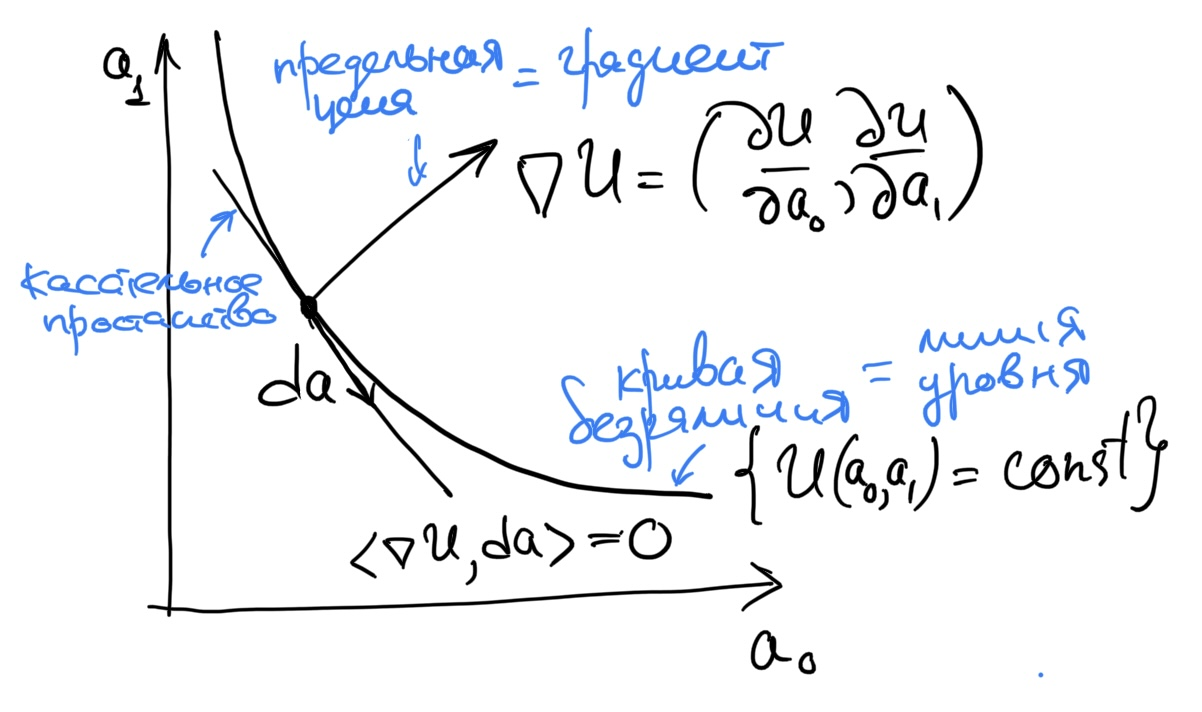
\includegraphics[width=1.0\textwidth]{2_figs/utility.jpeg}

\end{columns}


\end{frame}



\begin{frame}{Пример: CES-функция полезности}
CES-функция (constant elasticity of substitution) 
    $$
    u(x,y) = (\alpha x^{1/\rho} + \beta y^{1/\rho})^\rho 
    $$
$$
E = \frac{d \log(x/y)}{ d \log(u'_x/u'_y)} = \frac{1}{1-\rho}
$$
    
\begin{itemize}
    \item $\rho=1$: $u(x,y) = \alpha x + \beta y $
    \item $\rho=-\infty$: $u(x,y) = min(\alpha x,\beta y)$
    \item $\rho=0$: $u(x,y) = x^{\alpha}y^{\beta}$ (функция Кобба-Дугласа)
    
\end{itemize}
    
\end{frame}


\begin{frame}{Пример: work-life balance}

Work-life balance — это разделение личной и профессиональной жизни, которое помогает им взаимно друг друга поддерживать. Из-за развития технологий, достиженческой культуры, которая постоянно мотивирует добиваться больших и лучших результатов, и быстро меняющихся правил и условий труда именно навык создания и поддержания баланса становится важным: если «перевешивает» одна часть жизни, страдает другая\footfullcite{sber_worklifebalance}.
    
\end{frame}


\begin{frame}{Оптимальный выбор}

\begin{itemize}
    \item $x$ - количество часов работы
    \item $y$ - количество часов отдыха
    \item $u(x,y)$ - функция полезности
\end{itemize}

\begin{equation}
    \begin{cases}
      u(x,y) \to max\\
        x+ y = 24 
    \end{cases}
\end{equation}

$$
0 = \frac{d}{dx} u(x, 24-x) = u'_x - u'_y
$$

Равновесие: предельная польза от работы = предельной пользе от отдыха
\end{frame}


\begin{frame}{Общий случай: выбор при бюджетных ограничениях}

\begin{itemize}
    \item $a = (a_0, a_1 \ldots, a_n)$ - активы
    \item $p = (p_0, p_1, \ldots, p_n)$ - экзогенные цены
    \item $<p,a> = w$ - бюджетное ограничение
    \item $u(a)$ - функция полезности
\end{itemize}

Оптимизационная задача: $u(a) \to max \text{ при }  <p,a> = w $
$$
L(a,\lambda) = u(a) - \lambda(<p,a> - w)
$$
\begin{equation*}
    \begin{cases}
      \frac{\partial u}{\partial a} = \lambda p\\
      <p,a> = w
    \end{cases}
\end{equation*}


\end{frame}


\begin{frame}{Функция спроса и преобразование Лежандра}

Функция спроса:
$$
p \mapsto a(p) = \argmax_a (u(a) - \lambda(\langle p,a\rangle  - w)) 
$$
Преобразование Лежандра функции полезности:
$$
u^*(p) = max_a (u(a) - \lambda(\langle p,a\rangle - w)) 
$$
\begin{block}{Утверждение}
    $$
a = - \frac{1}{\lambda} \frac{\partial u^*(p)}{\partial p}
$$
\end{block}
Двойственность:
$$
p = \frac{1}{\lambda}\frac{\partial u(a)}{\partial a}
$$
    
\end{frame}

\section{Рынок нескольких агентов: равновесие по Парето}

\begin{frame}{Рынок нескольких агентов: равновесие по Парето}
  \centering
\Large Как моделировать обмен между агентами? 
\end{frame}

\begin{frame}{Рынок с одним активом}
\begin{columns}
    \column{0.5\linewidth}
\begin{itemize}
    \item Один товар: $x$
    \item Два участника: $u_1(x_1), u_2(x_2)$ - функции полезности 
    \item Только обмен товарами: $x_1 + x_2 = 1$
\end{itemize}


    \column{0.5\linewidth}
        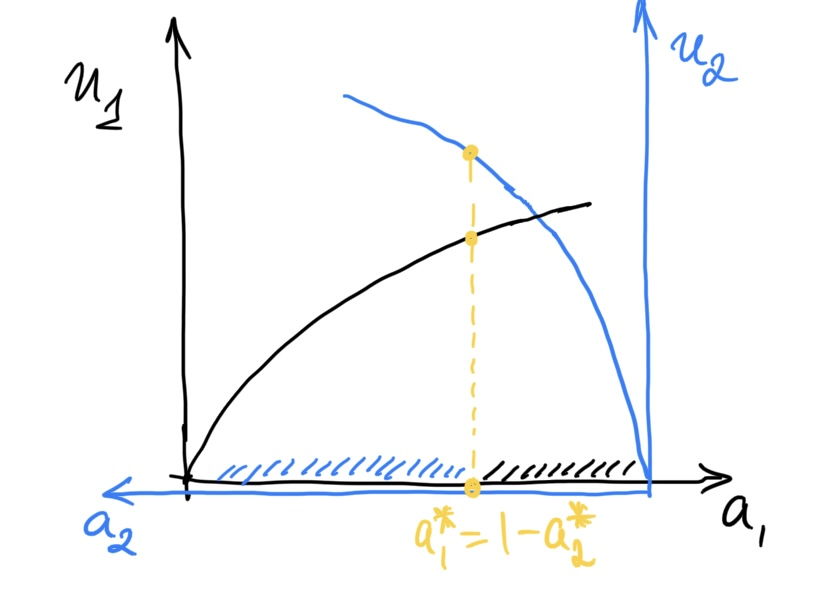
\includegraphics[width=1.0\textwidth]{2_figs/1asset.jpeg}


\end{columns}


Нет взаимовыгодного обмена - рынок в равновесии
\end{frame}

\begin{frame}{Рынок с двумя акт.: Ящик Эджворта (Edgeworth box)}

\begin{columns}
    \column{0.5\linewidth}
\begin{itemize}
    \item Два товара: $(x,y)$
    \item Два участника: $u_1(x_1,y_1), u_2(x_2,y_2)$ - функции полезности 
    \item Только обмен товарами: $x_1 + x_2 = 1$,  $y_1 + y_2 = 1$
\end{itemize}


    \column{0.5\linewidth}
        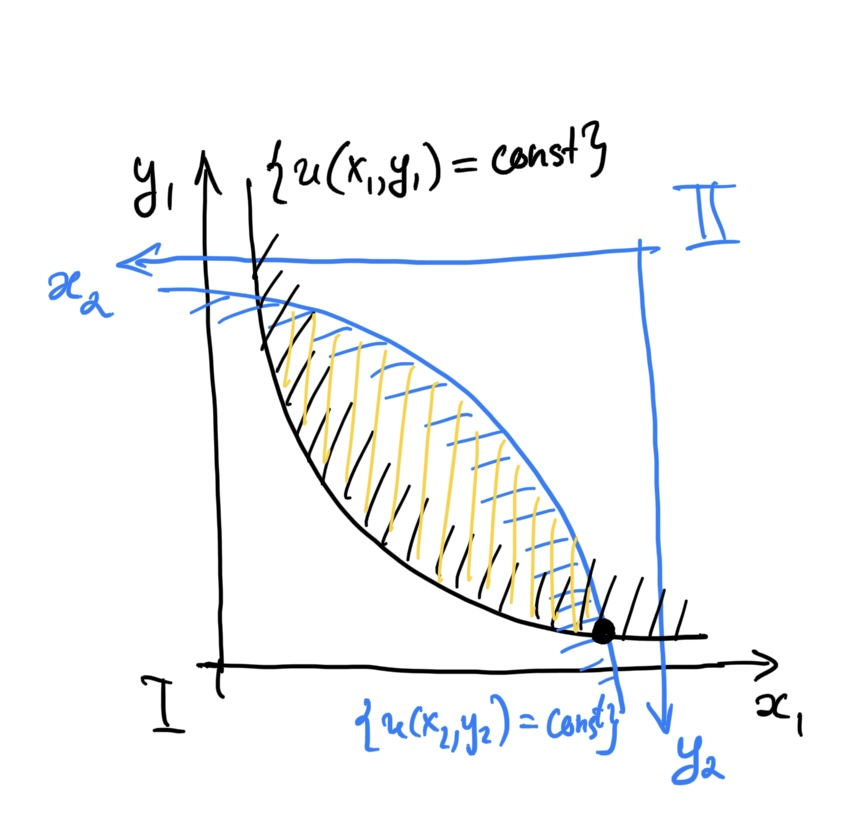
\includegraphics[width=1.0\textwidth]{2_figs/edgeworth.jpeg}


\end{columns}

\end{frame}

\begin{frame}{Парето эффективное распределение активов}

\begin{columns}
    \column{0.5\linewidth}
Контактная кривая: 
\begin{itemize}
    \item Нельзя улучшить полезность одного не уменьшая полезность другого
    \item Множество преобладающих распределений пусто
    \item Множество с отсутствием мотивации для торговли
    \item $MRS_1 = MRS_2$ 
\end{itemize}


    \column{0.5\linewidth}
        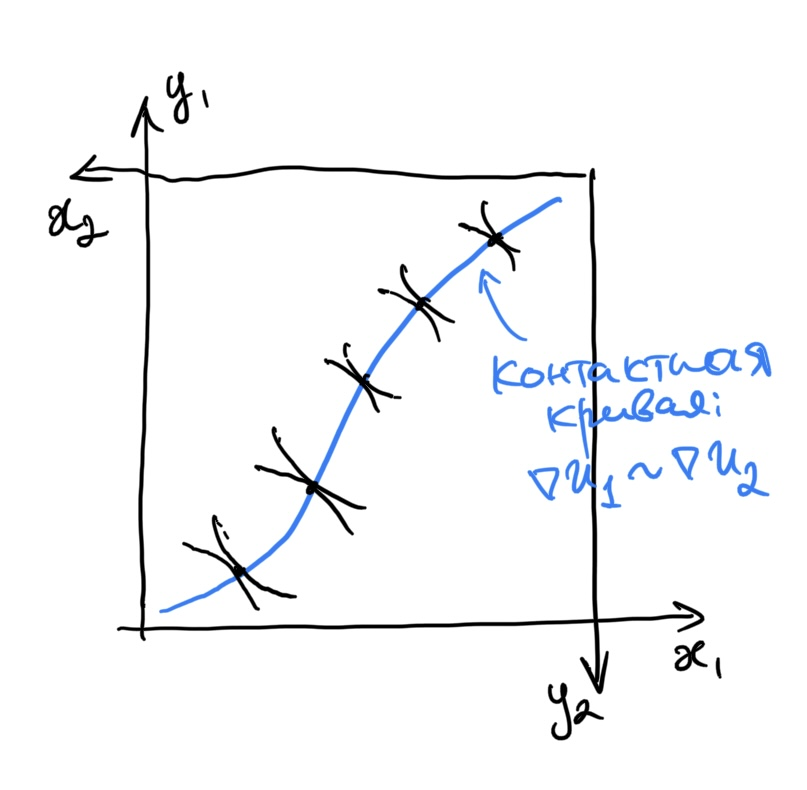
\includegraphics[width=1.0\textwidth]{2_figs/contact.jpeg}


\end{columns}
\end{frame}

\begin{frame}{Общий случай Парето эффективности}

Зададим покомпонентный (частичный!) порядок на векторах $a,b\in \R^k$:
$$
a\leq b \Leftrightarrow a_i \leq b_i, \quad\quad  a<b \Leftrightarrow  a\leq b \land a\neq b
$$

\begin{block}{Определение} 
Максимальное распределение $c^* = (c_1, \ldots, c_k)$ относительно порядка $<$ называется эффективным по Парето, то есть
$$
\nexists c: u(c) > u(c^*)
$$
$u(c) = (u_1(c), \ldots, u_k(c))$.
\end{block}

Нельзя улучшить аллокацию не дискриминируя никакого агента 
    
\end{frame}



\begin{frame}{Рынок совершенной конкуренции}
\begin{itemize}
    \item Агенты оптимизируют полезность при данных ценах (price-takers)
    $$
    p \mapsto c_j(p) = \argmax( u_j(c_j)|  <p,\Delta c_j(p)>=0)   
    $$
    \item Формируют кривые спроса и предложения:
    $$
    \Delta c_j(p) = c_j(p) - c^0_j 
    $$
    \item Цена которая клирит рынок - равновесие:
    $$
    \Delta c_1(p) = \Delta c_2(p)
    $$
    
\end{itemize}


\end{frame}

\begin{frame}{Фундаментальные теоремы экономики(1/3)}


\begin{block}{Первая фундаментальная теорема экономики}
    Конкурентное равновесие - Парето оптимально
\end{block}
\begin{columns}
    \column{0.5\linewidth}
        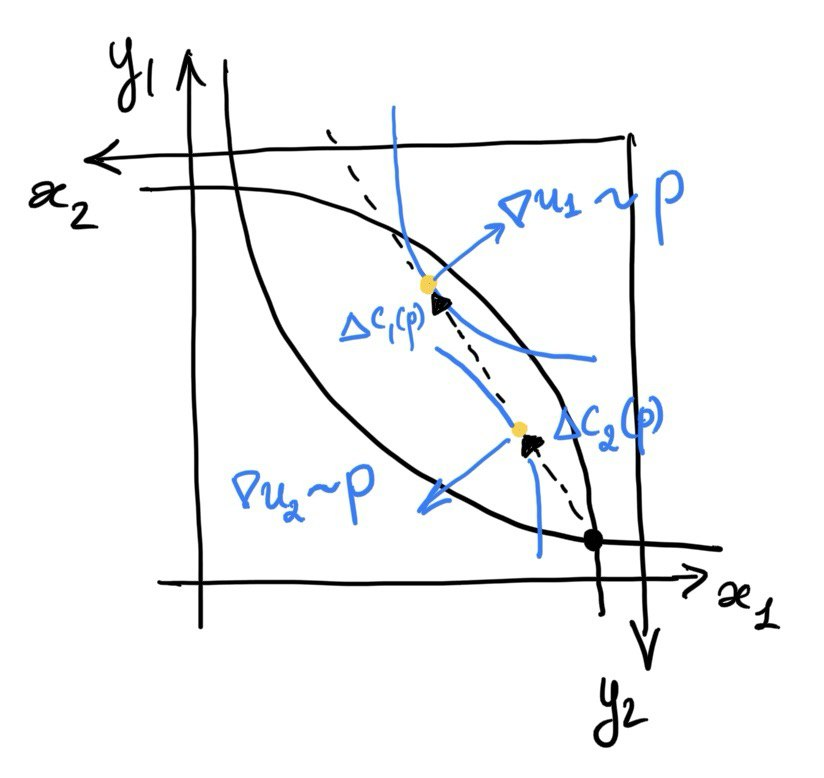
\includegraphics[width=1.0\textwidth]{2_figs/edgeworth_1ft_neq.jpg}


    \column{0.5\linewidth}
        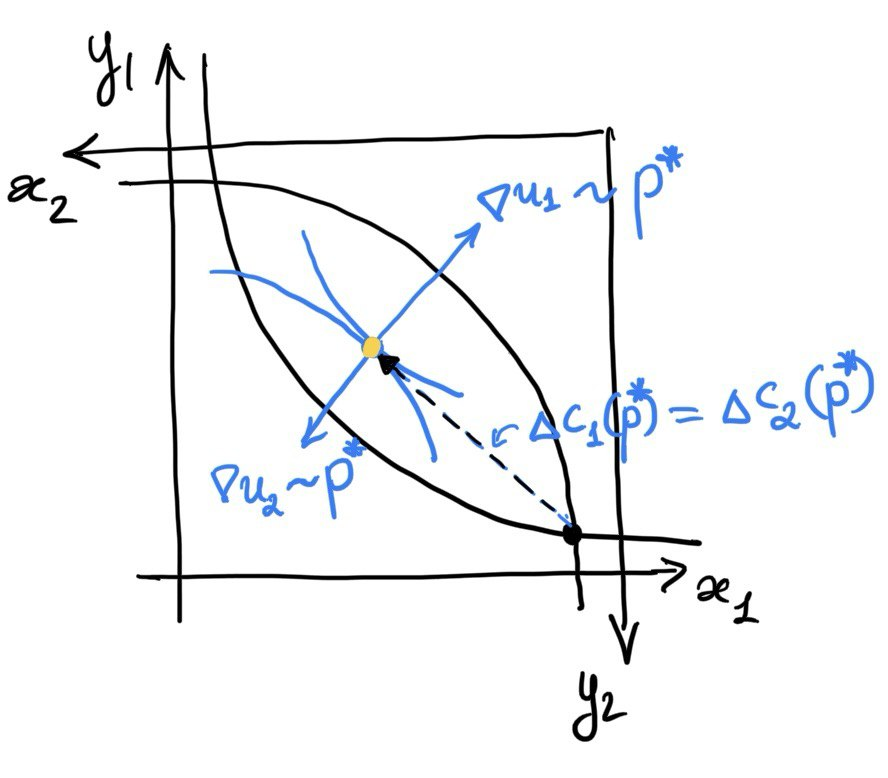
\includegraphics[width=1.0\textwidth]{2_figs/edgeworth_1ft.jpg}


\end{columns}


\end{frame}

\begin{frame}{Фундаментальные теоремы экономики(2/3)}

\begin{columns}
    \column{0.5\linewidth}
\begin{block}{Вторая фундаментальная теорема экономики}
    Любое Парето оптимальное распределение достижимо через трансферты
\end{block}


    \column{0.5\linewidth}
        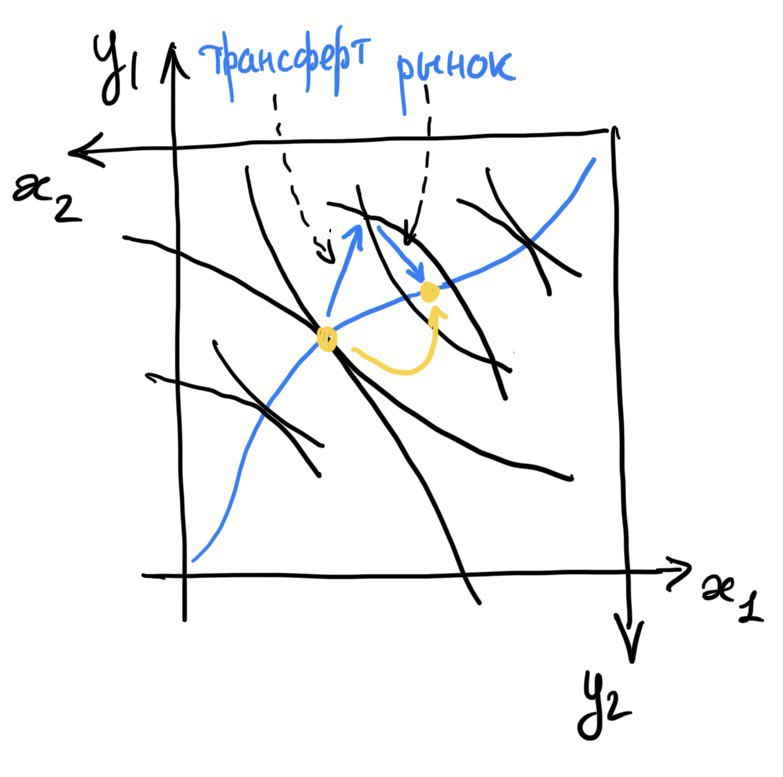
\includegraphics[width=1.0\textwidth]{2_figs/edgeworth_trans.jpg}


\end{columns}


\end{frame}


\begin{frame}{Фундаментальные теоремы экономики(3/3)}

\begin{block}{Агрегированная функция полезности}
    Рынок совершенной конкуренции нескольких агентов равносилен рынку одного агента
\end{block}

\end{frame}



\section{Рынок с асимметрией информации: теория игр}

\begin{frame}{Рынок с асимметрией информации: равновесие Нэша и дизайн механизмов}
  \centering
\Large Как моделировать асимметрию информации? 
\end{frame}

\begin{frame}{Дискриминирующее равновесие}

\begin{columns}
    \column{0.6\linewidth}
\begin{itemize}
    \item Два товара: $(x,y)$
    \item Два участника: $u_1(x_1,y_1), u_2(x_2,y_2)$ - функции полезности 
    \item Только обмен товарами: $x_1 + x_2 = 1$,  $y_1 + y_2 = 1$
    \item Полезность известна только агентам
    \item Первый сообщает ``дискриминирующую'' функцию полезности, второй - собственную
\end{itemize}



    \column{0.5\linewidth}
        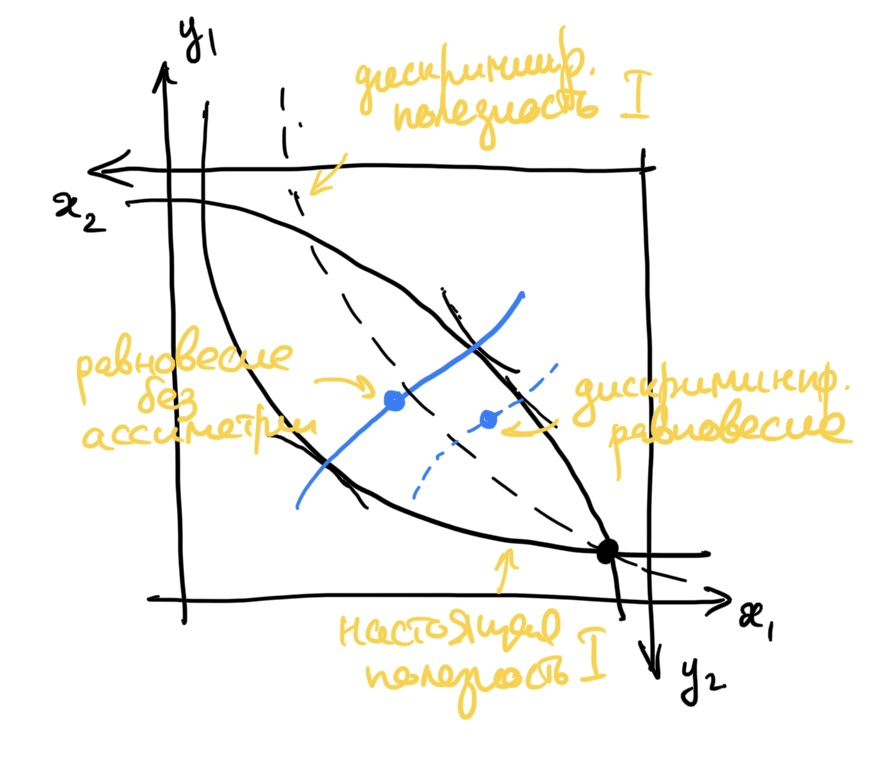
\includegraphics[width=1.0\textwidth]{2_figs/as.jpeg}


\end{columns}
\end{frame}

\begin{frame}{Игра в цыпленка}

Правда: сообщить собственную функцию полезности

Ложь: сообщить дискриминирующую функцию полезности

\begin{block}{Утверждение}
Рынок равносилен игре в цыпленка:
\begin{table}
    \centering
    \begin{tabular}{ccc}
         & Правда & Ложь\\
        Правда & $(\frac12,\frac12)$ &  $(\frac15,\frac35)$\\
        Ложь & $(\frac35,\frac15)$  & $(0,0)$ \\
    \end{tabular}
\end{table}

\end{block}
    
\end{frame}




\section{Рынок с неопределенностью: неприятие риска}

\begin{frame}{Рынок с неопределенностью: теория ожидаемой полезности и неприятие риска}
  \centering
\Large Как моделировать предпочтения в условиях неопределенности? 
\end{frame}


\begin{frame}{Санкт-петербургский парадокс}
    Игра:
    \begin{itemize}
        \item орел: выигрыш 1, решка: продолжаем
        \item орел: выигрыш 2, решка: продолжаем
        \item орел: выигрыш 4, решка: продолжаем
        \item ...
    \end{itemize}
    Сколько готовы заплатить за участие в такой игре?
\end{frame}

\begin{frame}{Санкт-петербургский парадокс}
    \begin{itemize}
        \item $F=1$ c вероятностью $\frac12$ 
        \item $F=2$ c вероятностью $\frac14$ 
        \item $F=4$ c вероятностью $\frac18$ 
        \item ...
    \end{itemize}

\pause
    $$
    \E F  = 1 \cdot \frac12 + 2\cdot\frac14 + 4\cdot\frac18 +\ldots = \frac12 + \frac12 + \frac12 \ldots = \infty 
    $$
\end{frame}


\begin{frame}{Однопериодная модель финансового рынка}

\begin{columns}
    \column{0.7\linewidth}
\begin{itemize}
\item один актив, но в разных состояниях 
\item $t=0$ - текущее состояние рынка
\item $t=1$ - $n$ состояний рынка
\item $p_1, \ldots, p_n$ - экзогенные вероятности состояний
\item $(a_0,a_1,\ldots, a_n)$ - вектор активов (потребления в каждом состоянии)
\end{itemize}

    \column{0.3\linewidth}
        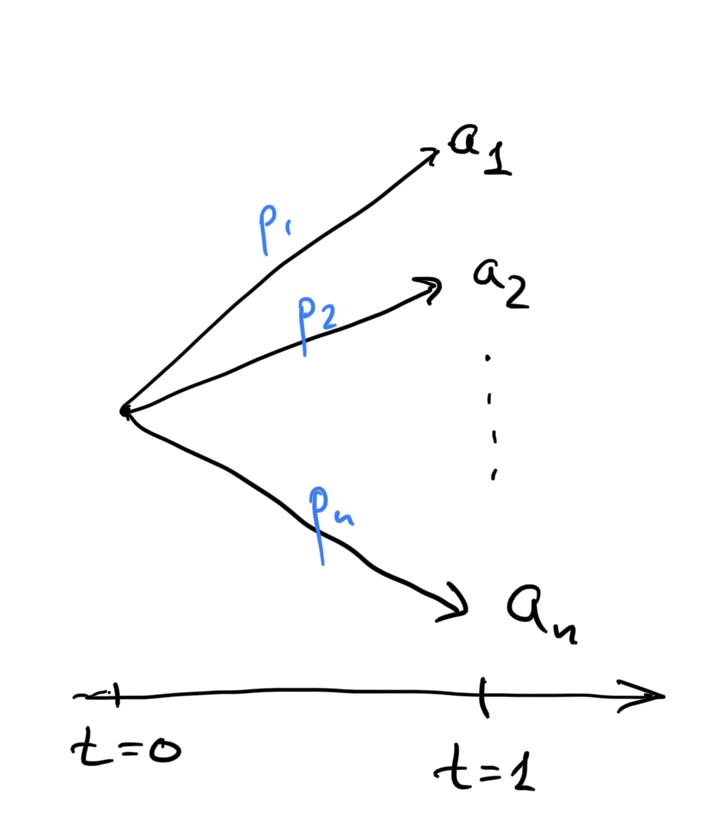
\includegraphics[width=1.0\textwidth]{2_figs/oneperiod.jpeg}


\end{columns}

\centering

\

\

Как сравнивать альтернативы $a \preceq  b$?

\pause
Ответ: $U(a) \leq U(b)$

Проблема: $U: \R^{n+1} \to \R$ и $n=\infty$ 
   
\end{frame}

\begin{frame}{Теория ожидаемой полезности}

Можно ли упростить $U(a)$?

\pause

Ответ (теория ожидаемой полезности): 
$$
U(a) = \E u(\alpha) = \sum_{j=1}^n p_j u(a_j) 
$$
\begin{equation*}\textbf{}
    \alpha = \begin{cases}
        a_1, p_1\\
        \ldots\\
        a_n, p_n
    \end{cases}    
\end{equation*}


   
\end{frame}


\begin{frame}{Стохастическое упорядочивание}

Задача: сравнить две случайные величины $\xi$ и $\eta$?

\pause

\begin{itemize}
    \item Стохастическое упорядочивание нулевого порядка
$$
\xi \preceq \eta \Leftrightarrow \text{supp}(f_\xi) \leq \text{supp}(f_\eta)
$$

\item Стохастическое упорядочивание первого порядка
$$
\xi \preceq \eta \Leftrightarrow F_\xi(x) \geq F_\eta(x)
$$

\item Стохастическое упорядочивание второго порядка
$$
\xi \preceq \eta \Leftrightarrow \int_{-\infty}^x F_\xi(y)dy \geq \int_{-\infty}^x F_\eta(y)dy
$$

\item ...
\end{itemize}
\end{frame}


\begin{frame}{Стохастическое упорядочивание первого порядка}
\begin{itemize}
\item $
\xi \preceq \eta \Leftrightarrow F_\xi(x) \geq F_\eta(x)
$
\item $\E u(\xi) \leq \E u(\eta)$ для любой неубывающей $u$

\item $\xi + \delta = \eta$, $\delta > 0$

\end{itemize}

\end{frame}

\begin{frame}{Стохастическое упорядочивание второго порядка}
\begin{itemize}
\item $
\xi \preceq \eta \Leftrightarrow F_\xi(x) \geq F_\eta(x)
$
\item $\E u(\xi) \leq \E u(\eta)$ для любой неубывающей и вогнутой $u$

\item $\xi + \delta = \eta$, $\E(\delta|\eta)=0$

\end{itemize}

\end{frame}

\begin{frame}{Теория ожидаемой полезности}
\begin{itemize}
\item (Рациональность) $\preceq$ - транзитивно и полно 
\item (Незасисимость) $a\preceq b \Rightarrow a + c \preceq b + c\  \forall c$ 
\item (Непрерывность) $a\preceq b \preceq c \Rightarrow \exists p:  b \sim (1-p)a + pc$  

\begin{block}{Теорема (Нейман -  Моргенштерн)}
    $\exists u:  a\preceq b \Leftrightarrow \E u(\alpha) \leq \E u(\beta)$
\end{block}

\end{itemize}

\end{frame}


\begin{frame}{Неприятие риска}

\begin{block}{Теорема}
    Неприятие риска $\Leftrightarrow$ Вогнутость функции полезности
    $$
    \E u(\xi) \leq u(\E \xi) \Leftrightarrow u''\leq 0
    $$
\end{block}

\end{frame}

\begin{frame}{Риск премия}

$$
\E u(\xi) = u(\E\xi - \pi)
$$
$$
\pi \approx \frac12 \alpha \sigma^2 
$$
$$
\alpha(x) = - \frac{u''(x)}{u'(x)}
$$


\end{frame}



\end{document}